\chapter*{Diagram benchmark tests}

In this section we list the topologically distinct contraction diagrams that 
are needed for doing spectroscopy on hadrons. We restrict ourselves to meson- 
and baryon-states and we only include diagrams that are needed for 1-1, 1-2 and 
2-2 scattering.
The intention is to see which way of evaluating the diagram yields the best 
performance. As we will see, the performance is very dependent on the order of 
contractions, so knowing which one is the fastest is important.

\begin{table}[]
	\centering
	\label{my-label}
	\begin{tabular}{@{}lcll@{}}
		\toprule
	Diagram	& Character rep. & Contraction pattern & Time \\ \midrule
	\parbox{1em}{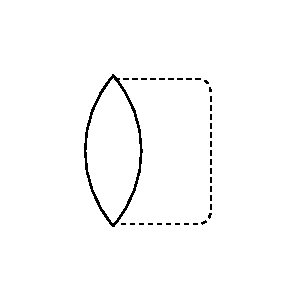
\includegraphics[width=2cm]{Aaa}}& $\tens{A}{_a_a}$ & 
	$\tens{A}{_a_a}$ & \SI{53(9)}{\micro s} \\
	\parbox{2cm}{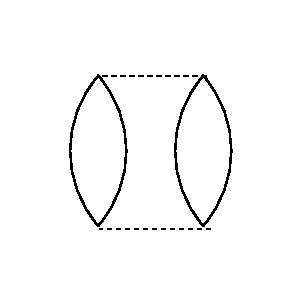
\includegraphics[width=2cm]{AabBab}} & 
	$\tens{A}{_a_b}\tens{B}{_a_b}$ & $\tens{A}{_a_b}\tens{B}{_a_b}$ & 
	\SI{0.37(10)}{\milli s}\\ 
	\parbox{2cm}{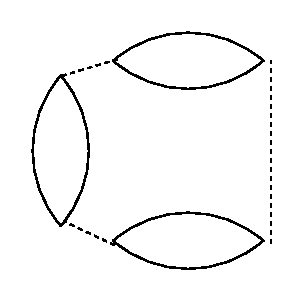
\includegraphics[width=2cm]{AabBbcCac}} & 
	$\tens{A}{_a_b}\tens{B}{_b_c}\tens{C}{_a_c}$ & 
	\parbox[c]{3cm}{$\tens{A}{_a_b}\tens{B}{_b_c} \rightarrow 
	\tens{D}{_a_c}$\\$\tens{D}{_a_c}\tens{C}{_a_c}$}  & 
	\SI{1.3(13)}{\milli s}\\
	\parbox{2cm}{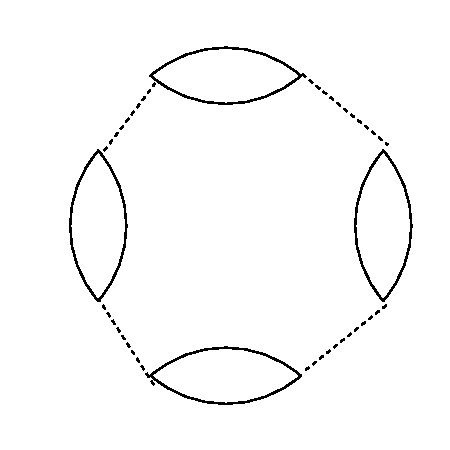
\includegraphics[width=2cm]{AabBbcCcdDad}} & 
	$\tens{A}{_a_b}\tens{B}{_b_c}\tens{C}{_c_d}\tens{D}{_a_d}$ & 
	\parbox[c]{3cm}{$\tens{A}{_a_b}\tens{B}{_b_c} \rightarrow 
		\tens{E}{_a_c}$\\$\tens{E}{_a_c}\tens{C}{_c_d}\rightarrow 
		\tens{F}{_a_d}$\\$\tens{F}{_a_d}\tens{D}{_a_d}$}  & 
	\SI{1.5(9)}{\milli s}\\
	\parbox{2cm}{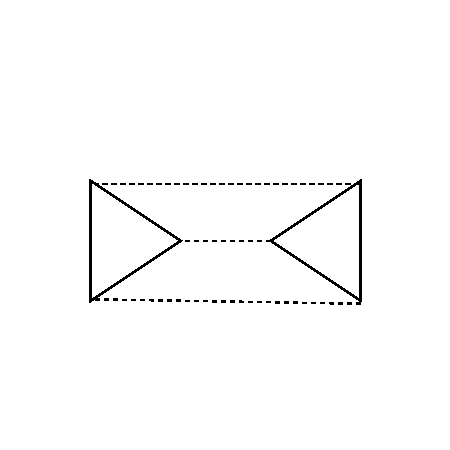
\includegraphics[width=2cm]{AabcBabc}} & 
	$\tens{A}{_a_b_c}\tens{B}{_a_b_c}$ & 
	\parbox[c]{3cm}{$\tens{A}{_a_b_c}\tens{B}{_a_b_c}$}  & 
	\SI{13.2(7)}{\milli s}\\
	\parbox{2cm}{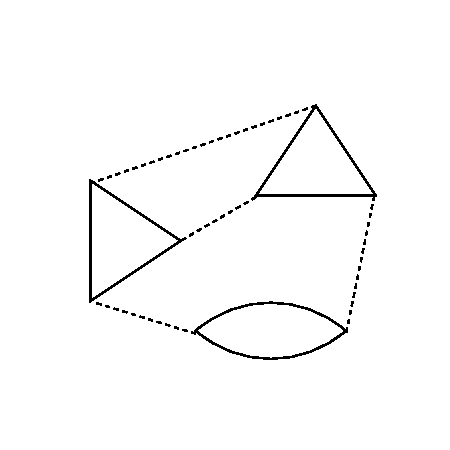
\includegraphics[width=2cm]{AabcBabdCcd}} & 
	$\tens{A}{_a_b_c}\tens{B}{_a_b_d}\tens{C}{_c_d}$ & 
	\parbox[c]{3cm}{$\tens{A}{_a_b_c}\tens{B}{_a_b_d} \rightarrow 
	\tens{D}{_c_d}$\\$\tens{D}{_c_d}\tens{C}{_c_d}$}  & 
	\SI{0.739(5)}{s}\\
	& 
	& 
	\parbox[c]{3cm}{$\tens{A}{_a_b_c}\tens{C}{_c_d} \rightarrow 
	\tens{D}{_a_b_d}$\\$\tens{D}{_a_b_d}\tens{B}{_a_b_d}$}  & 
	\SI{65(5)}{\milli s}\\
	 \bottomrule
	\end{tabular}
\end{table}

\begin{table}[]
	\centering
	\label{my-label}
	\begin{tabular}{@{}lcll@{}}
		\toprule
		Diagram	& Character rep. & Contraction pattern & Time \\ \midrule
		\parbox{2cm}{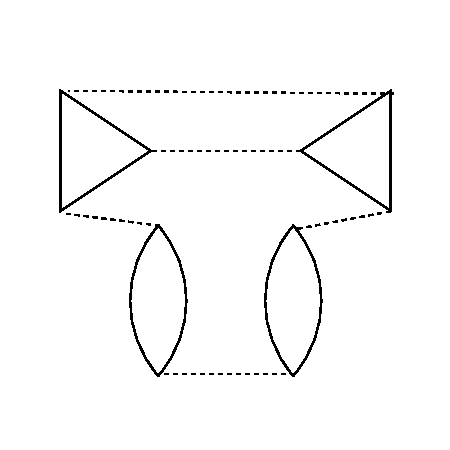
\includegraphics[width=2cm]{AabcBabdCceDde}} & 
		$\tens{A}{_a_b_c}\tens{B}{_a_b_d}\tens{C}{_c_e}\tens{D}{_d_e}$ & 
		\parbox[c]{3cm}{$\tens{A}{_a_b_c}\tens{B}{_a_b_d} \rightarrow 
			\tens{E}{_c_d}$\\$\tens{E}{_c_d}\tens{C}{_c_e}\rightarrow\tens{F}{_d_e}$\\
			$\tens{F}{_d_e}\tens{D}{_d_e}$}  & 
		\SI{0.738(5)}{s}\\
		& 
		& 
		\parbox[c]{3cm}{$\tens{A}{_a_b_c}\tens{C}{_c_e} \rightarrow 
			\tens{E}{_a_b_e}$\\$\tens{B}{_a_b_d}\tens{D}{_d_e}\rightarrow\tens{F}{_a_b_e}$\\
			$\tens{E}{_a_b_e}\tens{F}{_a_b_e}$}  & 
		\SI{0.119(16)}{s}\\ \\
		& 
		& 
		\parbox[c]{3cm}{$\tens{C}{_c_e}\tens{D}{_d_e} \rightarrow 
			\tens{E}{_c_d}$\\$\tens{A}{_a_b_c}\tens{E}{_c_d}\rightarrow\tens{F}{_a_b_d}$\\
			$\tens{F}{_a_b_d}\tens{B}{_a_b_d}$}  & 
		\SI{68.5(17)}{\milli s}\\
		\parbox{2cm}{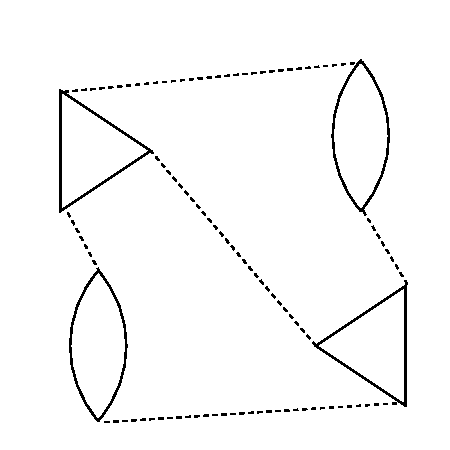
\includegraphics[width=2cm]{AabcBadeCbdDce}} & 
		$\tens{A}{_a_b_c}\tens{B}{_a_d_e}\tens{C}{_b_d}\tens{D}{_c_e}$ & 
		\parbox[c]{3cm}{$\tens{A}{_a_b_c}\tens{B}{_a_d_e} \rightarrow 
			\tens{E}{_b_c_d_e}$\\$\tens{E}{_b_c_d_e}\tens{C}{_b_d}\rightarrow\tens{F}{_c_e}$\\
			$\tens{F}{_c_e}\tens{D}{_c_e}$}  & 
		\SI{1.88(9)}{s}\\
		& 
		& 
		\parbox[c]{3cm}{$\tens{A}{_a_b_c}\tens{C}{_b_d} \rightarrow 
			\tens{E}{_a_c_d}$\\$\tens{E}{_a_c_d}\tens{B}{_a_d_e}\rightarrow\tens{F}{_c_e}$\\
			$\tens{F}{_c_e}\tens{D}{_c_e}$}  & 
		\SI{0.779(6)}{s}\\ \\
		& 
		& 
		\parbox[c]{3cm}{$\tens{A}{_a_b_c}\tens{C}{_b_d} \rightarrow 
			\tens{E}{_a_c_d}$\\$\tens{B}{_a_d_e}\tens{D}{_c_e}\rightarrow\tens{F}{_a_d_c}$\\
			$\tens{E}{_a_c_d}\tens{F}{_a_d_c}$}  & 
		\SI{87(8)}{\milli s}\\ \\
		& 
		& 
		\parbox[c]{3cm}{$\tens{A}{_a_b_c}\tens{C}{_b_d} \rightarrow 
			\tens{E}{_a_c_d}$\\$\tens{E}{_a_c_d}\tens{D}{_c_e}\rightarrow\tens{F}{_a_d_e}$\\
			$\tens{F}{_a_d_e}\tens{B}{_a_d_e}$}  & 
		\SI{87(3)}{\milli s}\\
		\parbox{2cm}{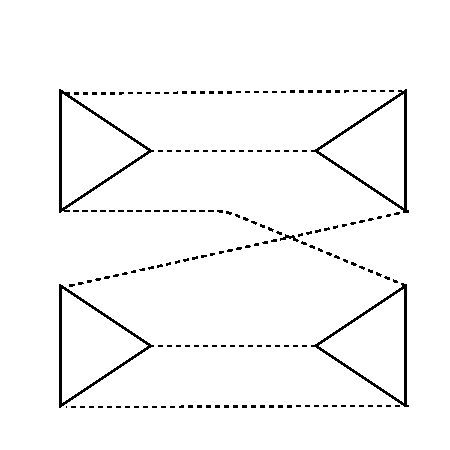
\includegraphics[width=2cm]{AabcBabdCdefDcef}} & 
		$\tens{A}{_a_b_c}\tens{B}{_a_b_d}\tens{C}{_d_e_f}\tens{D}{_c_e_f}$ & 
		\parbox[c]{3cm}{$\tens{A}{_a_b_c}\tens{B}{_a_b_d} \rightarrow 
			\tens{E}{_c_d}$\\$\tens{E}{_c_d}\tens{C}{_d_e_f}\rightarrow\tens{F}{_c_e_f}$\\
			$\tens{F}{_c_e_f}\tens{D}{_c_e_f}$}  & 
		\SI{0.762(9)}{s}\\
		& 
		& 
		\parbox[c]{3cm}{$\tens{A}{_a_b_c}\tens{B}{_a_b_d} \rightarrow 
			\tens{E}{_c_d}$\\$\tens{C}{_d_e_f}\tens{D}{_c_e_f}\rightarrow\tens{F}{_d_c}$\\
			$\tens{E}{_c_d}\tens{F}{_d_c}$}  & 
		\SI{1.500(4)}{s}\\ \\
		 & 
		 & 
		\parbox[c]{3cm}{$\tens{A}{_a_b_c}\tens{D}{_c_e_f} \rightarrow 
		\tens{E}{_a_b_e_f}$\\$\tens{B}{_a_b_d}\tens{C}{_d_e_f}\rightarrow\tens{F}{_a_b_e_f}$\\
		$\tens{E}{_a_b_e_f}\tens{F}{_a_b_e_f}$}  & 
		\SI{4.55(4)}{s}\\ \\
		& 
		& 
		\parbox[c]{3cm}{$\tens{A}{_a_b_c}\tens{D}{_c_e_f} \rightarrow 
		\tens{E}{_a_b_e_f}$\\$\tens{E}{_a_b_e_f}\tens{B}{_a_b_d}\rightarrow\tens{F}{_e_f_d}$\\
		$\tens{E}{_e_f_d}\tens{C}{_d_e_f}$}  & 
		\SI{48.4(2)}{s}\\
		\bottomrule
	\end{tabular}
\end{table}